\section{New Series from Old}

Although the brute force method is a great starting point, we don't want to have to do that every time we want a power series for a function.  Now that we have a library of known power series to draw from, we wish to manipulate these to construct new series rather than starting from scratch every time.  We have four loose categories for finding new series from old:
\begin{itemize}
\item Substitution
\item Algebra 
\item Differentiation
\item Antidifferentiation
\end{itemize}

\begin{subsection}{Substitution}\label{PowerSeriesSubstitution}  Replacing $x$ in a known series by another expression is often useful.

\begin{example}{Variations on a Theme of Euler}
Suppose we wish to find the power series for the function $f(x)=e^{-2x}$.  We can take our known series for the exponential function, $$e^x=1+x+\frac{1}{2!}x^2+\frac{1}{3!}x^3+\cdots, $$ and substitute $-2x$ for each occurance of $x$.  Proceeding, we have 
\begin{align*}
e^{-2x}&=1+\left(-2x\right)+\frac{1}{2!}\left(-2x\right)^2+\frac{1}{3!}\left(-2x\right)^3+\cdots\\
&=1-2x+\frac{2^2}{2!}x^2-\frac{2^3}{3!}x^3+\cdots\\
&=\sum_{n=0}^\infty\left(-1\right)^n\frac{2^n}{n!}x^n.
\end{align*}\end{example}
\begin{exercise}{Checking Against Brute Force \Coffeecup}
Use the brute force method to find the first four coefficients of the power series for $f(x)=e^{-2x}$.  Confirm they match what we obtained above via substitution. \vspace*{2in}
\end{exercise}
\begin{exercise}{Practice with Substitution \Coffeecup \Coffeecup \Coffeecup}
\begin{itemize}
\item Find a power series and the IOC for $\sin(x-1)$ centered at 1.
\vspace*{1in}
\item Find a power series and the IOC for $\sin(2x)$ centered at 0.
\vspace*{1in}
\end{itemize}
\AnswerKeyEntry{If we substitute $x-1$ for $x$ in the power series for sine, we get  $\sin(x-1)=\Sigma_{n=0}^\infty (-1)^{n}\frac{1}{\left(2n+1\right)!}(x-1)^{2n+1}$.  Likewise, substituting $2x$ for $x$ in the power series for sine produces $\sin(2x)=\Sigma_{n=0}^\infty (-1)^{n}\frac{1}{\left(2n+1\right)!}(2x)^{2n+1}=\Sigma_{n=0}^\infty (-1)^{n}\frac{2^{2n+1}}{\left(2n+1\right)!}x^{2n+1}$.}
\end{exercise}

\begin{example}{Revisiting the Arc Length of a Hyperbola}
The binomial series gives us a method by which we can obtain a decimal approximation for the arc length of a hyperbola, as stated in Example \ref{ArcLength}.\ref{HyperBocaBola}.  In that example, we wished to compute 
the arc length of $$y=f(x)=\frac{1}{x}. $$ between $x=\frac{1}{2}$ and $x=1$.  Unfortunately, the arc length integral came out to the less than cooperative  $$L= \int_{x=1/2}^{x=1} \sqrt{1+\left( f'(x)\right)^2 } \dif x= \int_{x=1/2}^{x=1} \frac{\sqrt{1+x^4}}{x^2} \dif x. $$

The trick here is to rewrite the function $\sqrt{1+x^4}$ using the Binomial Series.  In this case, $m=1/2$ and the usual $x$ in the Binomial Series has $x^4$ substituted in.  Proceeding, we see that \begin{align*}
\sqrt{1+x^4}&=\left(1+x^4\right)^{1/2}\\
&=\binom{1/2}{0}+\binom{1/2}{1}\left(x^4\right)+\binom{1/2}{2}\left(x^4\right)^2+\binom{1/2}{3}\left(x^4\right)^3+\binom{1/2}{4}\left(x^4\right)^4+\cdots \\
&=1+\frac{\left(\frac{1}{2}\right)}{1!}x^4+\frac{\left(\frac{1}{2}\right)\left(-\frac{1}{2}\right)}{2!}x^8+\frac{\left(\frac{1}{2}\right)\left(-\frac{1}{2}\right)\left(-\frac{3}{2}\right)}{3!}x^{12}+\frac{\left(\frac{1}{2}\right)\left(-\frac{1}{2}\right)\left(-\frac{3}{2}\right)\left(-\frac{5}{2}\right)}{4!}x^{16}+\cdots \\
&=1+\frac{1}{2}x^4-\frac{1}{8}x^8+\frac{1}{16}x^{12}-\frac{5}{128}x^{16}+\cdots. \\
\end{align*}
Noticing that the $x$-values in the integral are all between $\frac{1}{2}$ and 1, the quantity $x^4$ will also be in that interval.  Since the IOC of the Binomial Series at $m=1/2$ is $[-1,1]$, it is safe to use the power series as a substitute for $\sqrt{1+x^4}$ in the integral.  We now evaluate the integral using the Binomial Series.
\begin{align*}
L&= \int_{x=1/2}^{x=1} \frac{\sqrt{1+x^4}}{x^2} \dif x \\
&=\int_{x=1/2}^{x=1} \frac{1+\frac{1}{2}x^4-\frac{1}{8}x^8+\frac{1}{16}x^{12}-\frac{5}{128}x^{16}+\cdots}{x^2} \dif x \\
&=\int_{x=1/2}^{x=1} \frac{1}{x^2}+\frac{1}{2}x^2-\frac{1}{8}x^6+\frac{1}{16}x^{10}-\frac{5}{128}x^{14}+\cdots \dif x \\
&=\left. -\frac{1}{x}+\frac{1}{2\cdot 3}x^3-\frac{1}{8\cdot 7}x^7+\frac{1}{16\cdot 11}x^{11}-\frac{5}{128\cdot 15}x^{15}+\cdots\right]_{x=1/2}^{x=1}\\
 &=\left(-1+\frac{1}{6}-\frac{1}{56}+\frac{1}{176}-\frac{5}{1920}+\cdots\right)-\left(-2+\frac{1}{6\cdot 2^3}-\frac{1}{56\cdot 2^7}+\frac{1}{176\cdot 2^{11}}-\frac{5}{1920\cdot 2^{15}}+\cdots\right)\\
 &\approx 1.13
\end{align*}
Note this approximation is computed by just adding the terms written above and throwing away all further terms!  
\end{example}

\begin{exercise}{Comparing Two Approximations \Coffeecup}
In the above example, we approximated the arc length of the section of the hyperbola by using finitely many terms from the Binomial Series.  How does it compare if you instead approximated that same arc length via a single line segment?

\vspace*{1in}
\end{exercise}

\end{subsection}

\begin{subsection}{Algebra} An enormous plethora of algebraic tricks are useful with regards to \partialfractions{finding power series} for functions.  Often one can get a lot of mileage out of just factoring and juggling constants.

\begin{example}{Variation on a Geometric Series}
Suppose we wish to find a power series for the function $f(x)=\frac{1}{1-x}$ centered at 3.  We begin by adding and subtracting 3 from $x$, and then proceed to get the geometric series in a form where we can use substitution. \begin{align*}
f(x)&=\frac{1}{1-x}\\
&=\frac{1}{1-\left(x-3+3\right)}\\
&=\frac{1}{1-\left(x-3\right)-3}\\
&=\frac{1}{-2-\left(x-3\right)}\\
&=\frac{1}{-2}\frac{1}{1+\frac{\left(x-3\right)}{2}}\\
&=-\frac{1}{2}\frac{1}{1-\left(-\frac{\left(x-3\right)}{2}\right)}\\
\end{align*}
The motivation for the steps above was to get the series in a form where we can now use substitution into the standard geometric series. Specifically, we substitute $\left(-\frac{\left(x-3\right)}{2}\right)$ in for every occurrence of $x$.  
\begin{align*}
f(x)&=-\frac{1}{2}\left(1+\left(-\frac{\left(x-3\right)}{2}\right)+\left(-\frac{\left(x-3\right)}{2}\right)^2+\left(-\frac{\left(x-3\right)}{2}\right)^3+\cdots\right) \\
&=-\frac{1}{2}+\frac{1}{2^2}\left(x-3\right)-\frac{1}{2^3}\left(x-3\right)^2+\frac{1}{2^4}\left(x-3\right)^3-\cdots.
\end{align*}

\begin{center}
	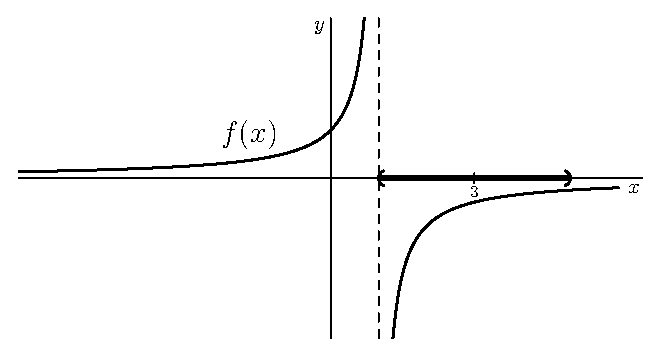
\includegraphics[width=300px]{ChapterPowerSeries/Figures/IntofConverg}
\end{center}
\end{example}
\begin{exercise}{Checking Against Brute Force \Coffeecup}
Once again, use the brute force method to find the first four coefficients of the power series for $f(x)=\frac{1}{1-x}$ centered at 3.  Confirm they match what we obtained above via algebra and substitution. \vspace*{2in}
\end{exercise}

\begin{exercise}{Practice with Algebra \Coffeecup \Coffeecup \Coffeecup}
\begin{itemize}
\item Find a power series and the IOC for $\frac{1}{x^2-x-12}$ centered at 0. ({\bf Hint:} Use PFD to split into two separate terms, each of which can then be turned into a power series using a variation on the geometric series.)

\vspace*{2in}

\item Find a power series and the IOC for $e^x$ centered at 2. ({\bf Hint:}  Replace $x$ by $(x-2)+2$ and then pull out an $e^2$.)

\vspace*{2in}

\item Find a power series and the IOC for $\sin(x)\cos(x)$ centered at 0. ({\bf Hint:} Avoid taking the nasty product of those two series by applying the sine double angle identity!)

\vspace*{2in}

\item Find a power series and the IOC for $\sin^2(x)$ centered at 0. ({\bf Hint:} Avoid taking the nasty product of sine with itself by applying the sine half angle identity!)

\vspace*{2in}
\item Find a power series and IOC for $\frac{1}{x}$ centered at $5$.

\vspace*{2in}
\end{itemize}
\AnswerKeyEntry{The power series $\frac{1}{x^2-x-12}=\Sigma_{n=0}^\infty  \left(\frac{-1}{21\cdot (-3)^n}-\frac{1}{28\cdot 4^n}\right)x^n$ has IOC (-3,3). The power series $\frac{1}{x}=\Sigma_{n=0}^\infty \frac{(-1)^n}{5^{n+1}}(x-5)^n$ has IOC (0,10).  It turns out these two examples generalize; for rational functions, the IOC will always just be the interval that goes from the center of the series outwards until it bumps into the nearest vertical asymptote!}
\end{exercise}
\end{subsection}

\begin{subsection}{Differentiation}  Often we differentiate a known \deriv{power series term-by-term} to find a new series.
\begin{exercise}{Practice with Differentiation \Coffeecup \Coffeecup \Coffeecup}
\begin{itemize}
\item Find a power series and IOC for $\frac{1}{x^2}$ centered at $5$. ({\bf Hint:} Use the answer from the last problem.)
 
\vspace*{2in}

\item Find a power series and IOC for $\frac{1}{x^3}$ centered at $5$. ({\bf Hint:} Use the answer from the last problem.)

\vspace*{2in}

\item Take the term-by-term derivative of the power series for $e^x$ centered at 0.  Verify that you do in fact get $e^x$ back!

\vspace*{2in}

\end{itemize}
\end{exercise}
\end{subsection}

\begin{subsection}{Antidifferentiation} Often we antidifferentiate a \antider{power series} term-by-term to \integ{find a new power series}.  You will have a ``$+C$'' to solve for by plugging in the center for $x$ after taking the antiderivative.  Notice that this $C$ is really just $a_0$, and plugging in the center for $x$ is just the first step of the brute force method. 

\begin{exercise}{Practice with Antidifferentiation \Coffeecup \Coffeecup \Coffeecup}
\begin{itemize}
\item Take the term-by-term antiderivative of the power series for $e^x$ centered at 0.  Verify that you do in fact get $e^x$ back!

\vspace*{2in}

\item Find a power series and IOC for $\ln(1-x)$ centered at zero.

\vspace*{2in}

\end{itemize}
\AnswerKeyEntry{Antidifferentiate the geometric series to sneak up on $\ln(1-x)$.}
\end{exercise}
\end{subsection}

\begin{exercise}{Four Different Methods for Finding the Same Power Series \Coffeecup \Coffeecup }
Compute the power series for the function $$f(x)=\frac{1}{(1-x)^2} $$
by following the four different methods outlined below:
\begin{enumerate}
\item Finding a power series using differentiation! \begin{itemize}
\item Write out the power series for $\frac{1}{1-x}$.
\item Differentiate both sides.
\vspace*{3in}
\end{itemize}

\item Finding a power series by multiplying together two known series! \begin{itemize}
\item Write out the power series for $\frac{1}{1-x}$.
\item Square both sides.  Note that this will involve a gigantic infinite FOIL on the right-hand side!
\vspace*{3in}
\end{itemize}

\item Finding a power series using long division! \begin{itemize}
\item Expand the denominator of $f(x)$, rewriting our function as $f(x)=\frac{1}{1-2x+x^2}$. 
\item Perform polynomial long division using the lowest degree term on each step to identify your quotient.
\vspace*{3in}
\end{itemize}

\item Finding a power series via brute force! \begin{itemize}
\item Write a general unknown series $f(x)=a_0+a_1x+a_2x^2+a_3x^3+\cdots$. 
\item Plug in zero and differentiate to repeatedly solve for the coefficients one at a time (our brute force method).
\vspace*{3in}
\end{itemize}
\AnswerKeyEntry{Each method should lead to $$\frac{1}{(1-x)^2}=1+2x+3x^2+4x^3+5x^4+\cdots  $$}
\end{enumerate}

\end{exercise}